\documentclass{article}
\usepackage[T1]{fontenc}
\usepackage{lmodern}
\usepackage{graphicx}
\usepackage{amsmath,amssymb}
\usepackage[a4paper,margin=2cm]{geometry}
\usepackage[absolute,overlay]{textpos}
\setlength{\TPHorizModule}{1mm}
\setlength{\TPVertModule}{1mm}
\usepackage[indonesian]{babel}
\usepackage{hyperref}
\setlength{\emergencystretch}{2em}
% unit: Halaman 32

\begin{document}

% === Halaman 32 (llm) ===

\section*{Feedback Shift Register (FSR)}

\begin{itemize}
    \item FSR adalah contoh sebuah \textit{keystream generator}.
    \item Umumnya diimplementasikan sebagai \textit{hardware}.
    \item FSR terdiri dari dua bagian: register geser (n bit) dan fungsi umpan balik
\end{itemize}

\vspace{50mm}

Fungsi umpan baik : $f(b_n, b_{n-1}, b_2, b_1)$
\[ b_n = f(b_n, b_{n-1}, b_2, b_1) \]

% deskripsi: Diagram blok Feedback Shift Register (FSR) yang menunjukkan register geser dengan bit b_n hingga b_1 dan kotak fungsi umpan-balik (feedback function) yang menerima input dari beberapa bit register dan memberikan output kembali ke bit b_n.
% bbox normalisasi: [0.1570, 0.4960, 0.7600, 0.7860]
\begin{textblock*}{126.63mm}(32.97mm,147.31mm)
\noindent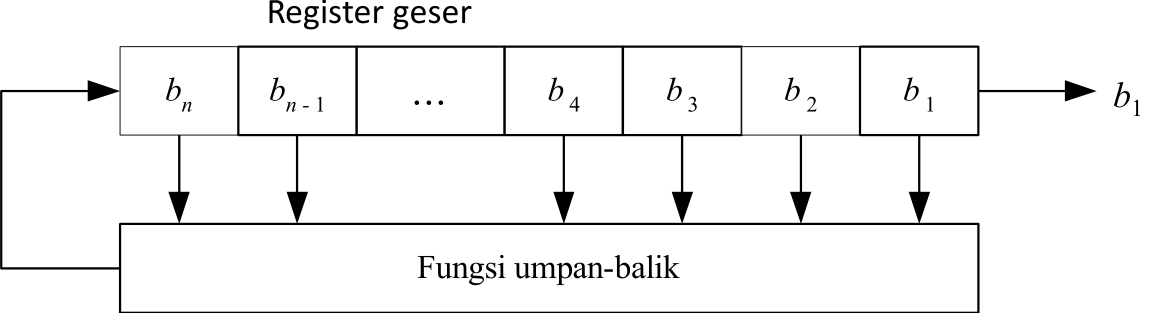
\includegraphics[width=126.63mm,height=86.13mm]{../../images/llm/page_032_img_01.png}%
\end{textblock*}

\end{document}
